\documentclass[11pt]{article}

\usepackage[margin=1in]{geometry}
\usepackage{amsmath,amssymb,amsthm}
\usepackage{enumitem}
\usepackage{listings}
\usepackage{xcolor}
\usepackage{booktabs}
\usepackage{tikz}
\usepackage{caption}
\usetikzlibrary{arrows.meta,positioning,calc,decorations.pathreplacing,fit,backgrounds}
\usepackage[hidelinks]{hyperref}

% ---- shared TikZ styles -------------------------------------------------
\tikzset{
  cell/.style   ={draw,minimum size=8mm,inner sep=0pt,thick},
  head/.style   ={cell,fill=gray!25},
  unit/.style   ={cell,fill=green!22},
  tail/.style   ={cell,fill=blue!12},
  vox/.style    ={circle,draw,fill=green!30,minimum size=3.4mm,inner sep=0pt},
  emptyvox/.style={circle,draw,dashed,minimum size=3.4mm,inner sep=0pt},
  vvec/.style   ={-{Stealth[length=2.6mm]},very thick,red!70!black},
  lbl/.style    ={font=\scriptsize},
}

\definecolor{codebg}{rgb}{0.96,0.96,0.97}
\definecolor{codekw}{rgb}{0.55,0.10,0.45}
\lstset{
  basicstyle=\ttfamily\small,
  backgroundcolor=\color{codebg},
  breaklines=true,
  frame=single,
  framesep=4pt,
  rulecolor=\color{lightgray},
  keywordstyle=\color{codekw}\bfseries,
  showstringspaces=false,
  columns=fullflexible,
}

\newtheorem{definition}{Definition}
\newtheorem{proposition}{Proposition}

\newcommand{\Z}{\mathbb{Z}}
\newcommand{\R}{\mathbb{R}}
\newcommand{\vv}{\mathbf{v}}
\newcommand{\pp}{\mathbf{p}}
\newcommand{\oo}{\mathbf{o}}
\newcommand{\loc}{\boldsymbol{\ell}}

\title{\textbf{Auto-Stack}\\[2pt]
\large Automatic Detection and Resizing of Repeating Structures in Voxel Builds}
\author{Nucleation resizer --- design notes}
\date{\today}

\begin{document}
\maketitle

\begin{abstract}
\emph{Auto-Stack} takes a Minecraft build---a redstone circuit, a display, or a
mechanical contraption such as a slimestone flying machine---detects the
repeating unit it is built from, and lets the user change how many times that
unit repeats, producing a new build. A 4-bit adder becomes 8-bit; a $32\times32$
screen becomes $64\times64$; an $N$-module bore head becomes $2N$. The whole
system reduces to one idea: a build is (locally) invariant under a lattice
translation $\vv$, and resizing means re-stamping its fundamental domain a
different number of times along $\vv$. This document describes how the period
$\vv$ is found, how the resize is performed for axis-aligned, diagonal, and
two-dimensional lattices, how the repeating cell is made self-contained and
re-stackable, and how non-block data (entities) is carried along.
\end{abstract}

\tableofcontents

\section{The core idea}

A build is a finite set of placed blocks
\[
G \;=\; \{\,(\pp, b) : \pp \in \Z^3,\ b \in \mathcal{B}\,\},
\]
mapping integer voxel positions to block states $b$ (a namespaced id plus
properties such as a comparator's \texttt{facing} or a repeater's
\texttt{delay}). A region of the build is \emph{periodic} with period
$\vv \in \Z^3$ if translating it by $\vv$ maps it onto itself:
\[
(\pp, b) \in G \;\Longleftrightarrow\; (\pp + \vv,\, b) \in G
\qquad\text{(away from the boundary).}
\]

The period $\vv$ need not be axis-aligned. A carry-chain adder whose bit-cells
march diagonally has $\vv=(2,-2,0)$; a vertically stacked datapath has
$\vv=(0,2,0)$; a flat display is periodic along \emph{two} independent vectors
$\vv_1,\vv_2$. Resizing is then mechanical: keep the irregular boundary, and
replace the periodic interior with however many copies of one period the user
asks for. Everything else in the system exists to (a) discover $\vv$ robustly,
(b) cut the build into period-cells correctly, and (c) re-stitch the cells so the
result is a valid, working build.

\section{Two levels of abstraction}\label{sec:levels}

The hard part of finding $\vv$ is that the right notion of ``repeating unit''
depends on what kind of build it is.

\begin{description}[leftmargin=1.4em]
\item[Computational redstone] (adders, displays). The functional structure is a
graph of redstone components. Two cells can be logically identical while their
voxels differ---signal-boosting repeaters are inserted at intervals, decoder
taps vary per row. Here the period must be found on the \emph{compiled graph},
not the voxels.

\item[Structural / mechanical] (flying machines, farms). These are mostly slime,
honey, pistons, and observers---blocks the redstone compiler barely models, so
the graph is nearly empty and useless. But the build's \emph{voxels} are
literally periodic: the bore head repeats as a block pattern. Here the period is
found directly on the voxels.
\end{description}

The system routes between the two with a cheap test on the block palette. Let
$\mathcal{C}$ be the set of ``computational'' blocks (wire, comparator, repeater,
torches, lamp, lever, button). Define the compute fraction
\[
\phi \;=\; \frac{\bigl|\{(\pp,b)\in G : b \in \mathcal{C}\}\bigr|}{|G|}.
\]
If $\phi < 0.35$ the build is treated as \emph{structural} and the period is
detected from voxels (\S\ref{sec:voxelperiod}); otherwise it is
\emph{computational} and the period is detected from the graph
(\S\ref{sec:graphperiod}). A flying machine has $\phi\approx0$; an adder has
$\phi\approx0.95$.

\section{Finding the period}

\subsection{From the graph: the invariance test}\label{sec:graphperiod}

For computational builds we extract the \emph{structural} compile graph---a
pre-fold graph in which every component (including each redstone-wire segment) is
its own node with a recorded voxel position $\mathrm{pos}(n)$ and a kind
$\mathrm{kind}(n)\in\{$Wire, Comparator, Repeater, Torch, Lamp, $\dots\}$.

\paragraph{Structural labels.} Each node is given a Weisfeiler--Lehman label that
captures its local role. Starting from $L_0(n)=\mathrm{kind}(n)$, we refine for a
few rounds,
\[
L_{r+1}(n) \;=\; \mathrm{hash}\Bigl(L_r(n),\ \{\!\{L_r(u) : u\to n\}\!\},\
\{\!\{L_r(w) : n\to w\}\!\}\Bigr),
\]
where $\{\!\{\cdot\}\!\}$ is a sorted multiset over in- and out-neighbours. Nodes
that play the same role in different bit-positions receive the same label.

\paragraph{Candidate direction.} The lattice direction is the dominant
displacement between equal-label nodes. We tally
$\pp(m)-\pp(n)$ over all pairs $m,n$ with $L(m)=L(n)$, take the most frequent
nonzero vector, and reduce it by the gcd of its components to a primitive
direction $\mathbf{d}$. This works for diagonal lattices: a displacement
$(2,-2,0)$ reduces to $\mathbf{d}=(1,-1,0)$.

\paragraph{The invariance test.} The dominant displacement is often a
\emph{sub-lattice} generator, not the true cell period. In a comparator-based
adder the comparators repeat every $2$ blocks, but a full bit-cell---comparators
\emph{and} the sparser output layer---repeats every $4$. To find the true period
we test invariance directly. For a candidate $\vv=m\,\mathbf{d}$, bucket every
node by its phase along $\vv$,
\begin{equation}\label{eq:phase}
k(n) \;=\; \left\lfloor \frac{(\pp(n)-\oo)\cdot\vv}{\lVert\vv\rVert^2} \right\rfloor,
\end{equation}
and let $H_k$ be the histogram of kinds in bucket $k$. Then
\begin{definition}
$\vv$ is a \emph{period} if there is a run of at least three consecutive interior
buckets with identical histograms, $H_k=H_{k+1}=\dots$.
\end{definition}
We take the smallest multiple $m=1,2,3,\dots$ of $\mathbf{d}$ that passes. This
rejects the comparator sub-lattice (its buckets alternate $H_k\neq H_{k+1}$) and
returns the genuine bit-cell period. Two implementation details matter: the
bucketing in \eqref{eq:phase} uses \emph{floor} division so each bucket is a
contiguous fundamental domain (rounding would split a cell across two buckets),
and the histogram comparison uses the coarse \emph{kind} label, not the full WL
label, because boundary effects make every node's WL label eventually unique.

\begin{figure}[ht]
\centering
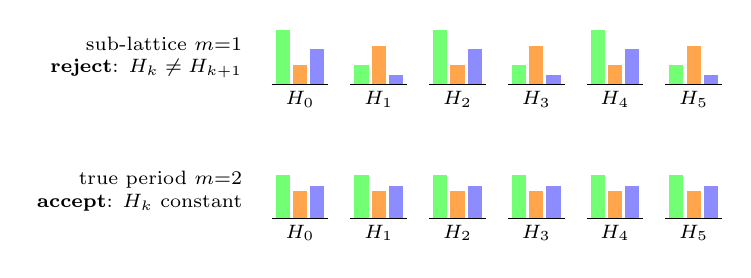
\begin{tikzpicture}[scale=1.0]
  % top row: sub-lattice -> histograms alternate -> rejected
  \node[lbl,align=right,anchor=east] at (-0.3,0.35)
        {sub-lattice $m{=}1$\\\textbf{reject}: $H_k\ne H_{k+1}$};
  \foreach \k/\ha/\hb/\hc in {0/0.7/0.25/0.45, 1/0.25/0.5/0.12, 2/0.7/0.25/0.45,
                              3/0.25/0.5/0.12, 4/0.7/0.25/0.45, 5/0.25/0.5/0.12}{
    \begin{scope}[shift={(\k*1.0,0)}]
      \fill[green!55] (0,0) rectangle (0.18,\ha);
      \fill[orange!70](0.22,0) rectangle (0.40,\hb);
      \fill[blue!45]  (0.44,0) rectangle (0.62,\hc);
      \draw[thin] (-0.05,0)--(0.67,0);
      \node[lbl] at (0.31,-0.18){$H_{\k}$};
    \end{scope}
  }
  % bottom row: true period -> identical histograms -> accepted
  \begin{scope}[yshift=-1.7cm]
    \node[lbl,align=right,anchor=east] at (-0.3,0.35)
          {true period $m{=}2$\\\textbf{accept}: $H_k$ constant};
    \foreach \k in {0,...,5}{
      \begin{scope}[shift={(\k*1.0,0)}]
        \fill[green!55] (0,0) rectangle (0.18,0.55);
        \fill[orange!70](0.22,0) rectangle (0.40,0.35);
        \fill[blue!45]  (0.44,0) rectangle (0.62,0.42);
        \draw[thin] (-0.05,0)--(0.67,0);
        \node[lbl] at (0.31,-0.18){$H_{\k}$};
      \end{scope}
    }
  \end{scope}
\end{tikzpicture}
\caption{The invariance test. Each bar group is the kind-histogram $H_k$ of phase
bucket $k$. A candidate that is only a sub-lattice generator (top: the
comparator step) produces histograms that alternate, so it is rejected; the
smallest multiple whose interior histograms are constant (bottom: the full
bit-cell) is the true period.}
\label{fig:invariance}
\end{figure}

\subsection{From the voxels: self-overlap}\label{sec:voxelperiod}

For structural builds there is no useful graph, so we find $\vv$ directly. For
each axis and each candidate period $T$ along it, slide the build by
$\vv=T\hat{e}_{\text{axis}}$ and measure how many overlapping voxels match:
\[
\mathrm{score}(\vv) \;=\; \bigl|\{\pp : (\pp,b)\in G,\ (\pp+\vv,b)\in G,\ \text{same id}\}\bigr|.
\]
The true period \emph{maximizes} the number of identical matches; a spurious
short shift matches only a handful of blocks. We keep the highest-scoring
$\vv$ whose match ratio exceeds $90\%$, breaking ties toward the shorter period.
On the $3{\times}7$ slimestone bore this returns $\vv=(6,0,0)$ at $97\%$
self-overlap---the bore module---with no graph involved at all.

\section{Resizing: lattice-vector stamping}\label{sec:stamp}

Once $\vv$ is known, the resize is a single mechanism that handles axis-aligned
and diagonal periods uniformly. Axis alignment is merely the special case where
$\vv$ has one nonzero component.

\paragraph{Cells.} Using the phase \eqref{eq:phase}, assign every voxel to a cell
$k$ and record its \emph{local} coordinate
\[
\loc(\pp) \;=\; \pp - k(\pp)\,\vv .
\]
Two voxels related by $+\vv$ get the same local coordinate, so for a periodic
region all interior cells share an identical local block set. Let $C_k$ be cell
$k$'s map from local coordinate to block.

\paragraph{Phase alignment.} The cell boundaries depend on where we place the
phase origin. We sweep the phase offset over one period and pick the alignment
that maximizes the longest run of byte-identical consecutive cells. That run is
the periodic interior; the cells before it are the \emph{head} (e.g.\ an adder's
input row, a machine's engine) and the cells after it the \emph{tail} (the
output cap, the bore's leading edge).

\paragraph{Reassembly.} To resize the interior to $N$ units, concatenate
\[
\underbrace{C_0,\dots,C_{s-1}}_{\text{head}},\
\underbrace{C_s,\;C_s,\;\dots,\;C_s}_{N\ \text{copies of the unit}},\
\underbrace{C_{s+r},\dots}_{\text{tail}},
\]
where $s$ is the run start and $r$ its original length, and stamp the $i$-th cell
in this sequence at offset $i\,\vv$:
\begin{equation}\label{eq:assemble}
G' \;=\; \bigl\{\,(\loc + i\,\vv,\ b) : (\loc,b)\in (\text{$i$-th cell}),\ i=0,1,2,\dots\,\bigr\}.
\end{equation}
Because the unit cell's blocks are byte-identical and placed at consecutive
multiples of $\vv$, adjacent stamped cells connect exactly as the original
interior did---the carry chain, the slime sheet, the bus all continue across the
seam. For a diagonal $\vv$ the tail simply slides diagonally; no special case is
needed.

\begin{figure}[ht]
\centering
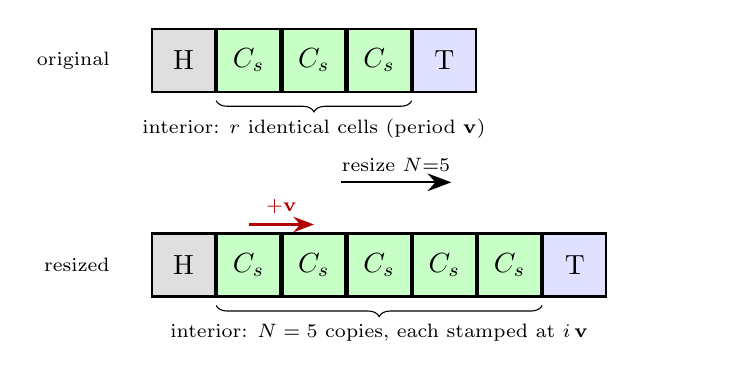
\begin{tikzpicture}[node distance=0pt]
  % original row
  \node[head]  (h0) at (0,0)   {H};
  \node[unit, right=of h0] (u1) {$C_s$};
  \node[unit, right=of u1] (u2) {$C_s$};
  \node[unit, right=of u2] (u3) {$C_s$};
  \node[tail, right=of u3] (t0) {T};
  \draw[decorate,decoration={brace,amplitude=4pt,mirror}]
        ($(u1.south west)+(0,-1mm)$) -- ($(u3.south east)+(0,-1mm)$)
        node[midway,below=3pt,lbl]{interior: $r$ identical cells (period $\vv$)};
  \node[left=4mm of h0,lbl,align=center]{original};
  % arrow
  \node (arr) at (6.6,-1.55) {};
  \draw[-{Stealth[length=3mm]},thick] (2.0,-1.55) -- (3.4,-1.55)
        node[midway,above,lbl]{resize $N{=}5$};
  % resized row
  \begin{scope}[yshift=-2.6cm]
    \node[head]  (H0) at (0,0)   {H};
    \node[unit, right=of H0] (U1) {$C_s$};
    \node[unit, right=of U1] (U2) {$C_s$};
    \node[unit, right=of U2] (U3) {$C_s$};
    \node[unit, right=of U3] (U4) {$C_s$};
    \node[unit, right=of U4] (U5) {$C_s$};
    \node[tail, right=of U5] (T0) {T};
    \draw[decorate,decoration={brace,amplitude=4pt,mirror}]
          ($(U1.south west)+(0,-1mm)$) -- ($(U5.south east)+(0,-1mm)$)
          node[midway,below=3pt,lbl]{interior: $N=5$ copies, each stamped at $i\,\vv$};
    \node[left=4mm of H0,lbl,align=center]{resized};
    \draw[vvec] ($(U1.north)+(0,1mm)$) -- ($(U2.north)+(0,1mm)$)
          node[midway,above,lbl,red!70!black]{$+\vv$};
  \end{scope}
\end{tikzpicture}
\caption{The resize is head\,+\,$N$ copies of the unit cell\,+\,tail, each cell
stamped at a successive multiple of the period $\vv$. The head (e.g.\ an adder's
input row, a machine's engine) and tail (output cap, leading edge) are kept
verbatim; only the interior count changes.}
\label{fig:resize}
\end{figure}

\begin{proposition}[Faithfulness]
Resizing to the original unit count ($N=r$) reproduces the input exactly.
\end{proposition}
This identity check is the system's main correctness guarantee: on the diagonal
adder, $N=7$ reproduces all $634$ blocks; on the $32^2$ frame buffer, $7{\times}7$
reproduces all $24906$.

\begin{figure}[ht]
\centering
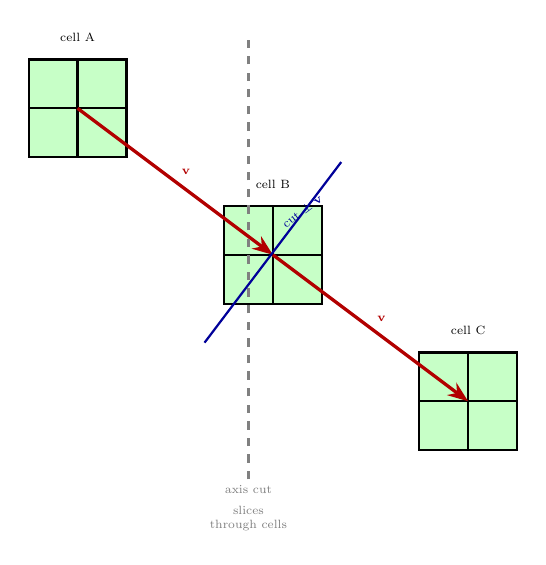
\begin{tikzpicture}[scale=0.62, every node/.style={transform shape}]
  % three diagonal cells (a staircase), each a 2x2 voxel cluster
  \foreach \cx/\cy/\name in {0/6/A, 4/3/B, 8/0/C}{
    \begin{scope}[shift={(\cx,\cy)}]
      \foreach \i in {0,1} \foreach \j in {0,1}
        \draw[fill=green!22,thick] (\i,\j) rectangle ++(1,1);
      \node[lbl] at (1,2.45) {cell \name};
    \end{scope}
  }
  % lattice vector v between cell anchors (down-right): (4,-3) here ~ diagonal
  \draw[vvec] (1,7) -- (5,4) node[midway,above right,lbl,red!70!black]{$\vv$};
  \draw[vvec] (5,4) -- (9,1) node[midway,above right,lbl,red!70!black]{$\vv$};
  % axis-aligned cut slices through a cell (bad)
  \draw[gray,dashed,thick] (4.5,-0.6) -- (4.5,8.4)
        node[pos=0.0,below,lbl,gray]{axis cut};
  \node[lbl,gray,align=center] at (4.5,-1.4){slices\\through cells};
  % correct cut: perpendicular to v, between cells (good)
  \draw[blue!60!black,thick] (3.6,2.2) -- (6.4,5.9);
  \node[lbl,blue!60!black,align=center,rotate=37] at (5.6,4.9){cut $\perp\vv$};
\end{tikzpicture}
\caption{A diagonal carry-chain adder: bit-cells step by $\vv=(2,-2,0)$. Bucketing
by phase along $\vv$ (the blue cut, perpendicular to $\vv$) separates the cells
cleanly; an axis-aligned slab (gray) cuts diagonally through every cell and
shears the carry chain. The same stamping that handles a vertical period
$(0,2,0)$ handles this one---axis alignment is just the case where $\vv$ has a
single nonzero component.}
\label{fig:diagonal}
\end{figure}

\section{Two-dimensional builds: displays}\label{sec:2d}

A flat display is periodic along two independent vectors $\vv_1,\vv_2$ (say the
screen's $Y$ and $Z$ axes), with the circuit depth $X$ aperiodic. Detection runs
the per-axis test on all three axes; if two axes are periodic we must still
decide whether it is a genuine 2D grid or merely a 1D diagonal lattice seen in
projection---a diagonal $\vv$ shows a period on \emph{both} of the axes it spans.

\paragraph{The grid-fill guard.} Bucket voxels into a 2D grid of cells
$(i,j)$ by phase along $\vv_1$ and $\vv_2$, and let the modal cell signature occur
$M$ times across an $I\times J$ grid. A true 2D grid fills a rectangle, so
$M$ is on the order of $I\cdot J$; a diagonal 1D lattice's cells lie on a line
$i+j=\text{const}$, so $M\approx\max(I,J)$. We declare 2D only when
\[
M \;\ge\; 2\max(I,J).
\]
This correctly keeps the diagonal adder one-dimensional while admitting the
frame buffer ($M=180$ on a $19\times18$ grid).

\begin{figure}[ht]
\centering
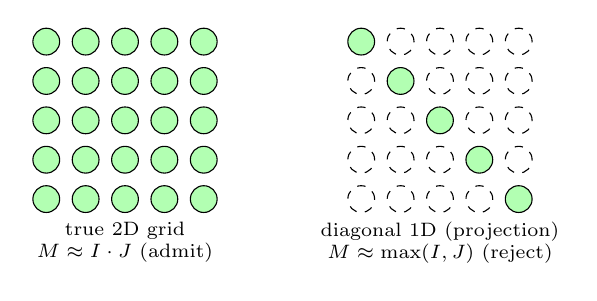
\begin{tikzpicture}[scale=0.5]
  % LEFT: true 2D grid -- cells fill the rectangle
  \begin{scope}
    \foreach \i in {0,...,4}\foreach \j in {0,...,4}
      \node[vox] at (\i,\j){};
    \node[lbl,align=center] at (2,-1.1){true 2D grid\\$M\approx I\cdot J$ (admit)};
  \end{scope}
  % RIGHT: diagonal 1D in projection -- cells on a line
  \begin{scope}[xshift=8cm]
    \foreach \i in {0,...,4}\foreach \j in {0,...,4}{
      \pgfmathtruncatemacro{\onLine}{\i+\j==4 ? 1 : 0}
      \ifnum\onLine=1 \node[vox] at (\i,\j){};
      \else \node[emptyvox] at (\i,\j){};\fi}
    \node[lbl,align=center] at (2,-1.1){diagonal 1D (projection)\\$M\approx\max(I,J)$ (reject)};
  \end{scope}
\end{tikzpicture}
\caption{The grid-fill guard. Counting how many cells share the modal signature
distinguishes a genuine 2D display (cells fill a rectangle) from a 1D diagonal
lattice whose cells, projected onto two axes, lie on a line $i+j=\text{const}$.
We declare 2D only when $M\ge 2\max(I,J)$.}
\label{fig:gridfill}
\end{figure}

\paragraph{Nine-slice tiling.} Resizing a screen to $M_1\times M_2$ interior tiles
is the 2D analogue of head/interior/tail: the four \emph{corners} stay fixed, the
four \emph{edges} (frame strips) scale 1D along the dimension they run, and the
\emph{interior} tiles in 2D. All nine regions follow one rule. Define a per-axis
remap from a new index to the original cell index it copies,
\[
\rho(i') = \begin{cases}
i' & i' < s \quad\text{(head: identity)}\\
s & s \le i' < s+M \quad\text{(interior: the unit)}\\
s + r + (i' - s - M) & \text{otherwise} \quad\text{(tail)}.
\end{cases}
\]
Then a new cell $(i',j')$ copies the original cell $(\rho_1(i'),\,\rho_2(j'))$,
stamped at $i'\vv_1 + j'\vv_2$. Corners hit (head,\,head), edges hit
(interior,\,boundary), and the interior hits (interior,\,interior)---one
expression covers them all.

\begin{figure}[ht]
\centering
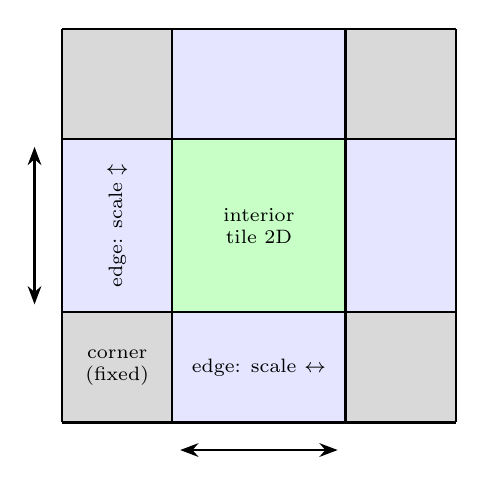
\begin{tikzpicture}[scale=1.0]
  % 3x3 nine-slice
  \def\a{0} \def\b{1.4} \def\c{3.6} \def\d{5.0}
  \foreach \x in {\a,\b,\c,\d} \draw[thick] (\x,0)--(\x,5);
  \foreach \y in {0,1.4,3.6,5}  \draw[thick] (0,\y)--(5,\y);
  % corners (fixed)
  \foreach \x/\y in {0/0, 3.6/0, 0/3.6, 3.6/3.6}
    \fill[gray!30] (\x,\y) rectangle ++(1.4,1.4);
  % center (tile 2D)
  \fill[green!22] (\b,\b) rectangle ++(2.2,2.2);
  % edges (scale 1D) light blue
  \fill[blue!10] (\b,0)   rectangle ++(2.2,1.4);
  \fill[blue!10] (\b,3.6) rectangle ++(2.2,1.4);
  \fill[blue!10] (0,\b)   rectangle ++(1.4,2.2);
  \fill[blue!10] (3.6,\b) rectangle ++(1.4,2.2);
  % redraw grid over fills
  \foreach \x in {\a,\b,\c,\d} \draw[thick] (\x,0)--(\x,5);
  \foreach \y in {0,1.4,3.6,5}  \draw[thick] (0,\y)--(5,\y);
  % labels
  \node[lbl,align=center] at (0.7,0.7){corner\\(fixed)};
  \node[lbl,align=center] at (2.5,2.5){interior\\tile 2D};
  \node[lbl,align=center] at (2.5,0.7){edge: scale $\leftrightarrow$};
  \node[lbl,align=center,rotate=90] at (0.7,2.5){edge: scale $\updownarrow$};
  % scaling arrows
  \draw[{Stealth}-{Stealth},thick] (1.5,-0.35)--(3.5,-0.35);
  \draw[{Stealth}-{Stealth},thick] (-0.35,1.5)--(-0.35,3.5);
\end{tikzpicture}
\caption{Nine-slice resize of a 2D display. The four corners are fixed; the top
and bottom edges scale horizontally and the left/right edges vertically (1D); the
interior tiles in both directions. The per-axis remap $\rho_1,\rho_2$ selects, for
each new cell, the original cell to copy---one rule for all nine regions.}
\label{fig:nineslice}
\end{figure}

\section{Self-contained cells: support-aware extraction}\label{sec:support}

Resizing only needs the period and the byte-identical slabs. Extracting a single
cell as a standalone, \emph{functional} build is harder, because a graph node's
voxel is not enough: a comparator rests on a block, a wall torch hangs off one,
and a wire is supported from below. Cutting a cell on a raw coordinate window
slices through these dependencies.

The fix is to grow the cell's voxel set by each component's \emph{functional
coupling}, which in redstone is directional, not a symmetric neighbourhood:

\begin{center}
\begin{tabular}{@{}ll@{}}
\toprule
component & structural blocks pulled in \\
\midrule
wire & support below; the horizontal neighbours it connects to \\
comparator / repeater & support below; the block it faces (output) and its back/side inputs \\
torch / wall torch & support or attachment block; the block it powers \emph{above} \\
lamp & none (self-supporting) \\
\bottomrule
\end{tabular}
\end{center}

\begin{figure}[ht]
\centering
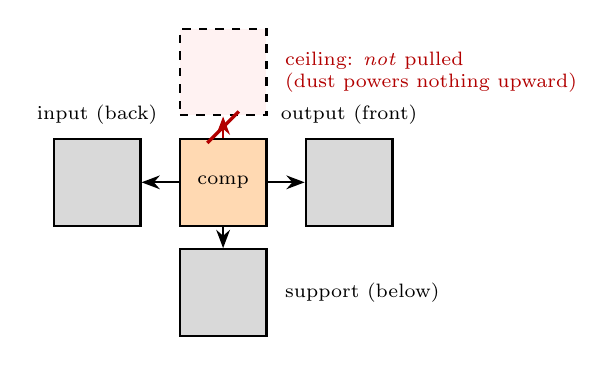
\begin{tikzpicture}[scale=1.0]
  % central comparator
  \node[cell,fill=orange!30,minimum size=11mm] (C) at (0,0) {\scriptsize comp};
  % support below (pulled)
  \node[cell,fill=gray!30,minimum size=11mm] (S) at (0,-1.4) {};
  \draw[-{Stealth},thick] (C.south) -- (S.north);
  \node[lbl,right=1mm of S]{support (below)};
  % front block = output (pulled), facing right
  \node[cell,fill=gray!30,minimum size=11mm] (F) at (1.6,0) {};
  \draw[-{Stealth},thick] (C.east) -- (F.west);
  \node[lbl,above=0.5mm of F]{output (front)};
  % back block = input (pulled)
  \node[cell,fill=gray!30,minimum size=11mm] (B) at (-1.6,0) {};
  \draw[-{Stealth},thick] (C.west) -- (B.east);
  \node[lbl,above=0.5mm of B]{input (back)};
  % ceiling NOT pulled
  \node[cell,draw,dashed,fill=red!5,minimum size=11mm] (U) at (0,1.4) {};
  \draw[-{Stealth},thick,red!70!black] (C.north) -- (U.south);
  \draw[red!70!black,very thick] ($(C.north)!0.5!(U.south)+(-2mm,-2mm)$)
        -- ++(4mm,4mm);
  \node[lbl,red!70!black,right=1mm of U,align=left]{ceiling: \emph{not} pulled\\(dust powers nothing upward)};
\end{tikzpicture}
\caption{Functional coupling is directional. A comparator's cell pulls in the
support block below it and the blocks it faces (output) and reads from
(input)---but \emph{not} the block above. A symmetric 6-neighbour ball would
wrongly drag in a ceiling.}
\label{fig:coupling}
\end{figure}

Crucially this is \emph{not} a 6-neighbour ball: dust does not power the block
above it, so a naive ball wrongly drags in a ``ceiling.'' With directional
coupling the extracted cell carries exactly the solids it depends on, all block
states are preserved losslessly, and the cell tiles back onto the original
$1{:}1$ under $\pm\vv$ shifts. Cross-cell blocks pulled in by the dilation are
duplicated harmlessly: stacking places identical blocks at identical coordinates.

\section{Carrying entities}\label{sec:entities}

Some builds place \emph{entities}---a slimestone bore drives instant block
updates with minecarts riding detector rails. Entities are not blocks; they have
floating-point positions and live outside the voxel grid. They tile with the same
lattice: each entity at world position $\pp_e$ is assigned to cell
$k=\lfloor(\pp_e-\oo)\cdot\vv/\lVert\vv\rVert^2\rfloor$, and in the reassembly
\eqref{eq:assemble} the entities of the cell copied into sequence slot $i$ are
re-emitted at $\pp_e + (i-k)\vv$. Boundary entities appear once; unit-cell
entities are replicated per stamped module. On the bore, three minecarts at
$x=1.5,7.5,13.5$ become $N{+}1$ carts on the extended rails, spacing preserved.

\section{Implementation and the web tool}

The detector and resizer are a single Python module (\texttt{resize\_lib.py})
built on the Nucleation library, which parses \texttt{.schem}/\texttt{.litematic}
files, exposes the structural compile graph, and meshes builds to textured glTF.
A dependency-free \texttt{http.server} front end lets the user drag in a file;
the back end returns circuit properties, a textured GLB preview (rendered in the
browser with three.js), and a resize control---one slider for 1D builds, two for
2D displays. Resizing returns a downloadable \texttt{.schem}.

\paragraph{A note on robustness.} Real files are messy. The bore litematic labels
its slime blocks \texttt{minecraft:slime}---the slime \emph{mob}'s id---rather
than \texttt{minecraft:slime\_block}; with no blockstate for that id the mesher
falls back to the entity model and renders mobs. The tool normalizes such
legacy/entity-colliding ids before meshing so the preview and the resized output
both show the correct block.

\section{The library API}\label{sec:api}

The pure-voxel core of this system---region-coverage detection
(\S\ref{sec:2d}) and lattice-vector resizing (\S\ref{sec:stamp})---is implemented
in the Nucleation Rust crate as the \texttt{autostack} module, behind a feature
flag of the same name, and exposed identically across the Python, WebAssembly,
and C/FFI bindings (checked by an API-parity tool). Detection returns a ranked
list of \texttt{Structure} descriptors---mode (\texttt{1d}/\texttt{2d}), period
vector(s), coverage, region bounding box, unit-cell bounding box, and a label;
resizing takes a structure (or its period vectors) plus the new cell count(s) and
returns a new schematic.

\begin{center}
\small
\begin{tabular}{@{}lll@{}}
\toprule
operation & Rust core & Python / WASM / FFI \\
\midrule
detect    & \texttt{detect\_structures(\&s)} & \texttt{detect\_structures()} \\
resize 1D & \texttt{resize\_1d(\&s, v, n)}    & \texttt{autostack\_resize\_1d(vx,vy,vz,n)} \\
resize 2D & \texttt{resize\_2d(\&s, v1, v2, n1, n2)} & \texttt{autostack\_resize\_2d($\dots$)} \\
\bottomrule
\end{tabular}
\end{center}

The Rust implementation is validated byte-for-byte against the reference
prototype on real builds: identical detected structures and identical resized
block sets for the 1D adder and the 2D screen. The advanced capabilities
(graph-based diagonal detection, near-periodic / booster resize, simulation-based
verification, support-aware single-cell extraction) remain in the prototype and
layer on behind the simulation feature.

\section{Scope and limitations}

\begin{itemize}[leftmargin=1.4em]
\item \textbf{Phase-projection vs.\ true interlock.} Bucketing by phase along
$\vv$ handles diagonal lattices and cells that snake in the plane perpendicular
to $\vv$. It does \emph{not} handle cells that interlock \emph{along} $\vv$
itself; that would require assigning cell membership by following the graph's
translation map combinatorially rather than by geometric projection.

\item \textbf{Near-periodic infrastructure.} Real displays are periodic at the
graph level but not byte-identical at the voxel level: signal boosters are
inserted by cumulative distance (with a heavier re-drive at the centre), and
address decoders grow as a $\log N$ demux tree. Pure tiling reproduces the pixel
array but not this infrastructure; resizing such a screen to a working larger one
needs parametric \emph{regeneration} of the boosters and decoder, which is
circuit synthesis rather than tiling.

\item \textbf{Functional verification.} The system guarantees the resized build
tiles byte-identically; it does not (currently) simulate the result to confirm
the carry propagates or the machine still flies. For clean lattices tiling
implies correctness, but this is inferred, not proven.

\item \textbf{Transparency.} The preview matches Nucleation's native renderer
(alpha-blended, double-sided, no depth write), which leaves cross-material
translucent z-ordering (e.g.\ slime against water) imperfect without
order-independent transparency.
\end{itemize}

\section*{Summary}
\addcontentsline{toc}{section}{Summary}
The entire system is one equation applied at two abstraction levels. Find the
translation $\vv$ under which the build is invariant---on the compile graph for
circuits (via an invariance test that rejects sub-lattices), on the raw voxels
for machines (via self-overlap). Cut the build into cells by phase along $\vv$,
keep the boundary, and re-stamp the interior cell $N$ times at multiples of
$\vv$. The same mechanism resizes a vertically stacked adder, a diagonal
carry-chain adder, a two-dimensional display, and a slimestone flying machine,
carrying support blocks and minecarts along with it.

\end{document}
